 %%%%%%%%%%%%%%%%%%%%%%%%%%%%%%%%%%%%%%%%%%%%%%%%%%%%%%%%%%%%%%%%%%%
%%%
%%%   Bachelor thesis pre-print 
%%%
%%%  English Title: 
%%%      LaTeX Template for Graduate Research Thesis
%%% 
%%%                                          written by Kentaro UNO 
%%%
%%%	 2020.01.08 Last modified by Kentaro UNO to set pBibtex function
%%%	 2020.01.24 Last modified by Kentaro UNO to desing as a template
%%%	 2022.12.26 Last modified by Kentaro UNO to build this template in overleaf
%%%
%%%%%%%%%%%%%%%%%%%%%%%%%%%%%%%%%%%%%%%%%%%%%%%%%%%%%%%%%%%%%%%%%%%%

%%%%%%%%%%%%%%%%%%%%%%%%%%%%%%%%%%%%%%%%
%%%  Texの汎用パッケージのロード
%%%%%%%%%%%%%%%%%%%%%%%%%%%%%%%%%%%%%%%%
\documentclass[a4paper,10pt,twocolumn]{jsarticle}
\renewcommand{\refname}{References}% <-- to make the bibliography section title show in English
\usepackage{color}
\usepackage{afterpage}
\usepackage{multicol}
\usepackage{nidanfloat}
\usepackage{amsmath} %AMSのLatex数学ライブラリ
\usepackage{amssymb} %AMSのLatex記号ライブラリ
\usepackage{comment}
\usepackage{setspace}
\usepackage{caption}
\usepackage{subcaption}
\usepackage[subrefformat=parens]{subcaption}
\usepackage{enumitem}
\usepackage{cite}

%%% Hyper link を使用するためのパッケージ added by Kentaro UNO 2020.3.21
\usepackage[dvipdfmx]{hyperref,graphicx}
% 日本語文字化け防止パッケージ
\usepackage{pxjahyper}
\hypersetup{% hyperrefオプションリスト
% setpagesize=true,
 pdfborder={2 2 1},
 colorlinks=true,
 linkcolor=black,
 citecolor=black,
 urlcolor=black,
%%% 下記,アンコメントでLinkのBoaderが点線四角になる
% pdfborderstyle=/S/D/D[3 2]/W 1,
%%% 下記,アンコメントでLinkのBoaderがアンダーラインになる
% pdfborderstyle={/S/U/W 1},
%%% その他色の調整など-->"\hypersetup option"で検索.
% linkcolor=blue,
% citecolor=red,
}
\usepackage{flushend} % added by Kentaro UNO 2022/02/28


%%%%%%%%%%%%%%%%%%%%%%%%%%%%%%%%%%%%%%%%
%%%  TeX macro command settings
%%%%%%%%%%%%%%%%%%%%%%%%%%%%%%%%%%%%%%%%
%%%%%%%%%%%%%%%%%%%%%%%%%%%%%%%%%%%%%%%%%%%%%%%%%%%%%%%%%%%%%%%%%%%%%%
%%
%%   macrosForEThesis.tex
%%   -------------------
%%
%%   Title: LaTeX macro file for the English Thesis
%%   
%%   
%%   Belief:
%%   1."Fig. 1: ~~~", "Table 1: ~~~" are for the figure and table citation.
%%   2. add the config to read the source code file (hello.c) and visualize it. 
%%
%%   Change Log:
%%   2020.11.26 Initial creation by Kentaro UNO
%%
%%   Contact:
%%   Please contact the author Kentaro UNO (unoken.astro@gmail.com) if
%%   you have a problem
%%
%%%%%%%%%%%%%%%%%%%%%%%%%%%%%%%%%%%%%%%%%%%%%%%%%%%%%%%%%%%%%%%%%%%%%%

%%% useful command
\newcommand{\n}{\nonumber \\}
\newcommand{\p}{\partial}
\newcommand{\bs}[1]{\boldsymbol{#1}}
\newcommand{\II}{I\negthinspace I}
\newcommand{\III}{I\negthinspace I\negthinspace I}
\newcommand{\mbm}[1]{\mbox{\protect \boldmath $#1$}}

%%%%%%%%%%%%%%%%%%%%%%%%%%%%%%%%%%%%%%%%
%%%  config for citation of figures, tables, and equations
%%%  to use English for all. 
%%%  2020.01.29 modified by Kentaro UNO
%%%%%%%%%%%%%%%%%%%%%%%%%%%%%%%%%%%%%%%%

%%% figure and table
\captionsetup{compatibility=false}
%
\renewcommand{\figurename}{Fig.~\hspace{-.2em}}   
\renewcommand{\tablename}{Table~\hspace{-.2em}}

\captionsetup[figure]{format=plain,labelformat=simple,labelsep=colon,font=small}
\captionsetup[table]{format=plain,labelformat=simple,labelsep=colon,font=small}

\newcommand{\bhline}[1]{\noalign{\hrule height #1}} % bhline command

%%% citation command for figures, tables, and equations
\newcommand{\fig}[1]{Fig.~\ref{#1}}
\newcommand{\subfig}[2]{Fig.~\ref{#1}\subref{#2}}
\newcommand{\fign}[1]{\ref{#1}}
\newcommand{\tb}[1]{Table~\ref{#1}}
\newcommand{\tabn}[1]{\ref{#1}}
\newcommand{\eq}[1]{Eq.~(\ref{#1})}
\newcommand{\eqn}[1]{(\ref{#1})}

%%% citation command for chapters, sections, and appendixes
\newcommand{\chap}[1]{Chap.~\ref{#1}}
\newcommand{\sect}[1]{Sect.~\ref{#1}}
\newcommand{\subsect}[1]{Sect.~\ref{#1}}
\newcommand{\app}[1]{Appnd. ~\ref{#1}}

%%% visualize a figure and table in a row
\makeatletter
\newcommand{\figcaption}[1]{\def\@captype{figure}\caption{#1}}
\newcommand{\tblcaption}[1]{\def\@captype{table}\caption{#1}}
\makeatother

%%%%%%%%%%%%%%%%%%%%%%%%%%%%%%%%%%%%%%%%
%%%  ソースコードの引用スタイルの設定
%%%  2020.01.24 added by Kentaro UNO
%%%%%%%%%%%%%%%%%%%%%%%%%%%%%%%%%%%%%%%%
\usepackage{listings} %日本語のコメントアウトをする場合はjlistingが必要
%ここからソースコードの表示に関する設定
\definecolor{gray}{rgb}{0.9,0.9,0.9}
\lstset{
  backgroundcolor=\color{gray}, % choose the background color; you must add \usepackage{color} or \usepackage{xcolor}; should come as last argument
  basicstyle={\small\ttfamily}, % the style of the fonts that are used for the code
  identifierstyle={\small}, % main()の''main''等のスタイル
  commentstyle={\small\itshape}, %//comment 等のスタイル
  keywordstyle={\small}, % int mainの''int''等のスタイル
  ndkeywordstyle={\small},
  stringstyle={\small\ttfamily},  % string literal style -> % printf(''Hello'')の''''で囲まれた部分のスタイル
  %frame={tb},
  breaklines=true, % sets automatic line breaking
  columns=[l]{fullflexible},
  numbers=left, % where to put the line-numbers; possible values are (none, left, right)
  numberstyle={\scriptsize}, % the style that is used for the line-numbers
  stepnumber=1, % the step between two line-numbers. If it's 1, each line will be numbered
  numbersep=1zw, % 行数字とコードの間のマージン
  xrightmargin=0zw, % 表示個所の右側マージン
  xleftmargin=2zw,  % 表示個所の左側マージン
  rulecolor=\color{black},         % if not set, the frame-color may be changed on line-breaks within not-black text (e.g. comments (green here))
  showspaces=false,                % show spaces everywhere adding particular underscores; it overrides 'showstringspaces'
  showstringspaces=false,          % underline spaces within strings only
  showtabs=false,                  % show tabs within strings adding particular underscores
  lineskip=-0.5ex % codeの行間の設定
}

\def\epsgaiji#1{\leavevmode\kern-0.025zw\raise-.37zh\hbox{%
  \epsfile{file=#1,width=1.05zw}}\kern-0.025zw}
%\newcommand{\dfrac}[2]{\frac{\displaystyle{#1}}{\displaystyle{#2}}}
\newcommand{\MARU}[1]{{\ooalign{\hfil#1\/\hfil\crcr\raise.167ex\hbox{\mathhexbox20D}}}}

%%%  % made a macrosForEThesis.tex to wrap the settings by Kentaro UNO 2020.1.28


%%%%%%%%%%%%%%%%%%%%%%%%%%%%%%%%%%%%%%%%
%%%  text lateral size 
%%%%%%%%%%%%%%%%%%%%%%%%%%%%%%%%%%%%%%%%
\oddsidemargin  -5.4mm    %% 左余白20mm
\evensidemargin -5.4mm    %% 左余白20mm
\textwidth 170mm    %% 右余白20mm
\columnsep 10mm     %% コラム間10mm

%%%%%%%%%%%%%%%%%%%%%%%%%%%%%%%%%%%%%%%%
%%%  text vertical size 
%%%%%%%%%%%%%%%%%%%%%%%%%%%%%%%%%%%%%%%%
\topmargin -5.4mm %% 上20mm
\headheight 0mm
\headsep 0mm
\textheight 257mm %%%% 297 - 20*2 = 257
\footskip 0mm

%%%%%%%%%%%%%%%%%%%%%%%%%%%%%%%%%%%%%%%%
%%%  文字横間隔,行間隔 
%%%%%%%%%%%%%%%%%%%%%%%%%%%%%%%%%%%%%%%%
\renewcommand{\baselinestretch}{0.83} %% すべての行間
\baselineskip 4.2mm     %% 連続する文章の行間
\kanjiskip=0.5pt plus 1pt minus 3pt %% 文字間隔
%\xkanjiskip=0.5pt plus 1pt minus 3pt  %% 文字間隔
\parindent 9pt        %% 段落の字下げ(9pt=1字分)
%\parskip 0.5mm       %% 段落の間隔 4.2mm - 9pt*0.3514 = 1.037

\textfloatsep 1.5mm     %%図表上下幅
\floatsep 1.5mm       %%図表上下幅
\intextsep 1.5mm     %%図表上下幅

\jot 0mm
\abovedisplayskip -5mm      %%数式上幅
\belowdisplayskip -5mm      %%数式下幅
\abovedisplayshortskip -5mm   %%数式上幅
\belowdisplayshortskip -5mm   %%数式上幅

%%%%%%%%%%%%%%%%%%%%%%%%%%%%%%%%%%%%%%%%
%%%  初期設定 
%%%%%%%%%%%%%%%%%%%%%%%%%%%%%%%%%%%%%%%%
\pagestyle{empty}
%%%%%%%%%%%%%%%%%%%%%%%%%%%%%%%%%%%%%%%%%%%%%%%%%%%%%%%%%%
\makeatletter
%........ {section}{1}{左から x mm}{上間隔 y mm}{下間隔 z mm}{フォントタイプ}}
\renewcommand{\section}{\@startsection{section}{1}{0mm}{2mm}{1mm}{\large\bf}}
\renewcommand{\subsection}{\@startsection{subsection}{2}{0mm}{1.5mm}{1mm}{\normalsize\bf}}
\renewcommand{\subsubsection}{\@startsection{subsubsection}{3}{0mm}{3mm}{1mm}{\small\bf}}
\makeatother
%%%%%%%%%%%%%%%%%%%%%%%%%%%%%%%%%%%%%%%%%%%%%%%%%%%%%%%%%%

%%%%%%%%%%%%%%%%%%%%%%%%%%%%%%%%%%%%%%%%
%%%  文書部分の開始 
%%%%%%%%%%%%%%%%%%%%%%%%%%%%%%%%%%%%%%%%
\begin{document}
\twocolumn[
\begin{center}
{~~~~~~~~~~~~~~~~~~~~~~~~~~~~~~~~~~~~~~~~~~~~~~~~~~~~~~~~Preprint of Graduation Study~~~~~~~~~~~~~~~~~~~~~~~~~~~~~~~Feb 2nd, 2024}\\
{\normalsize
~~~~~~~~~~~~~~~~~~~~~~~~~~~~~~~~~~~~~~~~~~~~~~~~~~~~~~~~~~~~~~~~~~~~~~~~~~~~~~~~~~~~~~~~~~~~~~~~~~~~~~~ \\}
{\normalsize
~~~~~~~~~~~~~~~~~~~~~~~~~~~~~~~~~~~~~~~~~~~~~~~~~~~~~~~~~~~~~~~~~~~~~~~~~~~~~~~~~~~~~~~~~~~~~~~~~~~~Name:~~~~~~~~~Tharit Sinsunthorn~~~~~~}\\
{\normalsize
~~~~~~~~~~~~~~~~~~~~~~~~~~~~~~~~~~~~~~~~~~~~~~~~~~~~~~~~~~~~~~~~~~~~~~~~~~~~~~~~~~~~~~~~~~~~~~~~~Supervisors:~~Prof. Kazuya Yoshida}\\
{\normalsize
~~~~~~~~~~~~~~~~~~~~~~~~~~~~~~~~~~~~~~~~~~~~~~~~~~~~~~~~~~~~~~~~~~~~~~~~~~~~~~~~~~~~~~~~~~~~~~~~~~~~~~~ \\}

\textbf{\large Title: Self-Recognition-based Motion Control of a Modular Legged Robot}\\
\end{center}
\vspace*{2zw}
]
%%% Section 1 %%%
\section{Introduction}\label{intro}
\indent
In the pursuit of lunar exploration, a modular legged robot, Moonbot,  was designed to transcend traditional boundaries in robotics. Moonbot integrates a self-recognition based system, allowing it to dynamically adapt to different configurations.

From the various innovative modularity concept on the legged robot \cite{snapbot1, snapbot2, modularrobot}, Moonbot seeks to improve the concept of modularity by combining with a general and higher level of legged robot control system design \cite{syropod}. Moonbot, as a result, inherits the adaptability and dynamically selecting control motions from a diversity of leg configurations, ranging from one to four. This self-awareness not only enhances Moonbot's locomotion capabilities but also broadens the scope for versatile applications in the challenging terrains of lunar exploration.

This thesis explains development of a modular control system for a reconfigurable legged robot.

%%% Section 2 %%%
\section{Modular Legged Robot:``Moonbot''}
Moonbot is the first version of a modular robot for the Moonshot project, "Self Evolving AI Robot System for Lunar Exploration and Human Outpost Construction" \cite{moonshotGoal3B}. The targets of this robot are self-reconfigurable and self-assembly abilities with the future implementation of Reinforcement Learning Algorithms for locomotion. 
Using internal sensors between main body and modular legs, Moonbot autonomously performs a real-time self-recognition system to identify the locomotion style fitting with the configuration.

Moonbot is PLA 3D-printed designed with a 20$\times$20 cm square shape, consisting of 4 magnetic connection ports at each corner. The electrical connection consists of U2D2, a USB communication converter for connecting with servo motors.   

There are four yaw-pitch-pitch modular legs for full assembly with 35 cm of length. Each of the legs is connected to the body via 8 pairs of radial Neodynium magnets, arranged in circular pattern as shown in \fig{fig1}\subref{subfig2}. The position control of Dynamixel XM430-W350-R servo motors, transferring the data via 3-pin TTL communication, are used to control the motion of the leg.

% The mass of the body is 840 grams and the mass of each legs is 530 grams. With the different numbers of module connection and combinations, Moonbot can identify the motion style of each connected leg to perform various kinds of locomotion.
%%%

%%%
\begin{figure}[t]
 \begin{subfigure}{0.23\textwidth}
 \begin{center}
  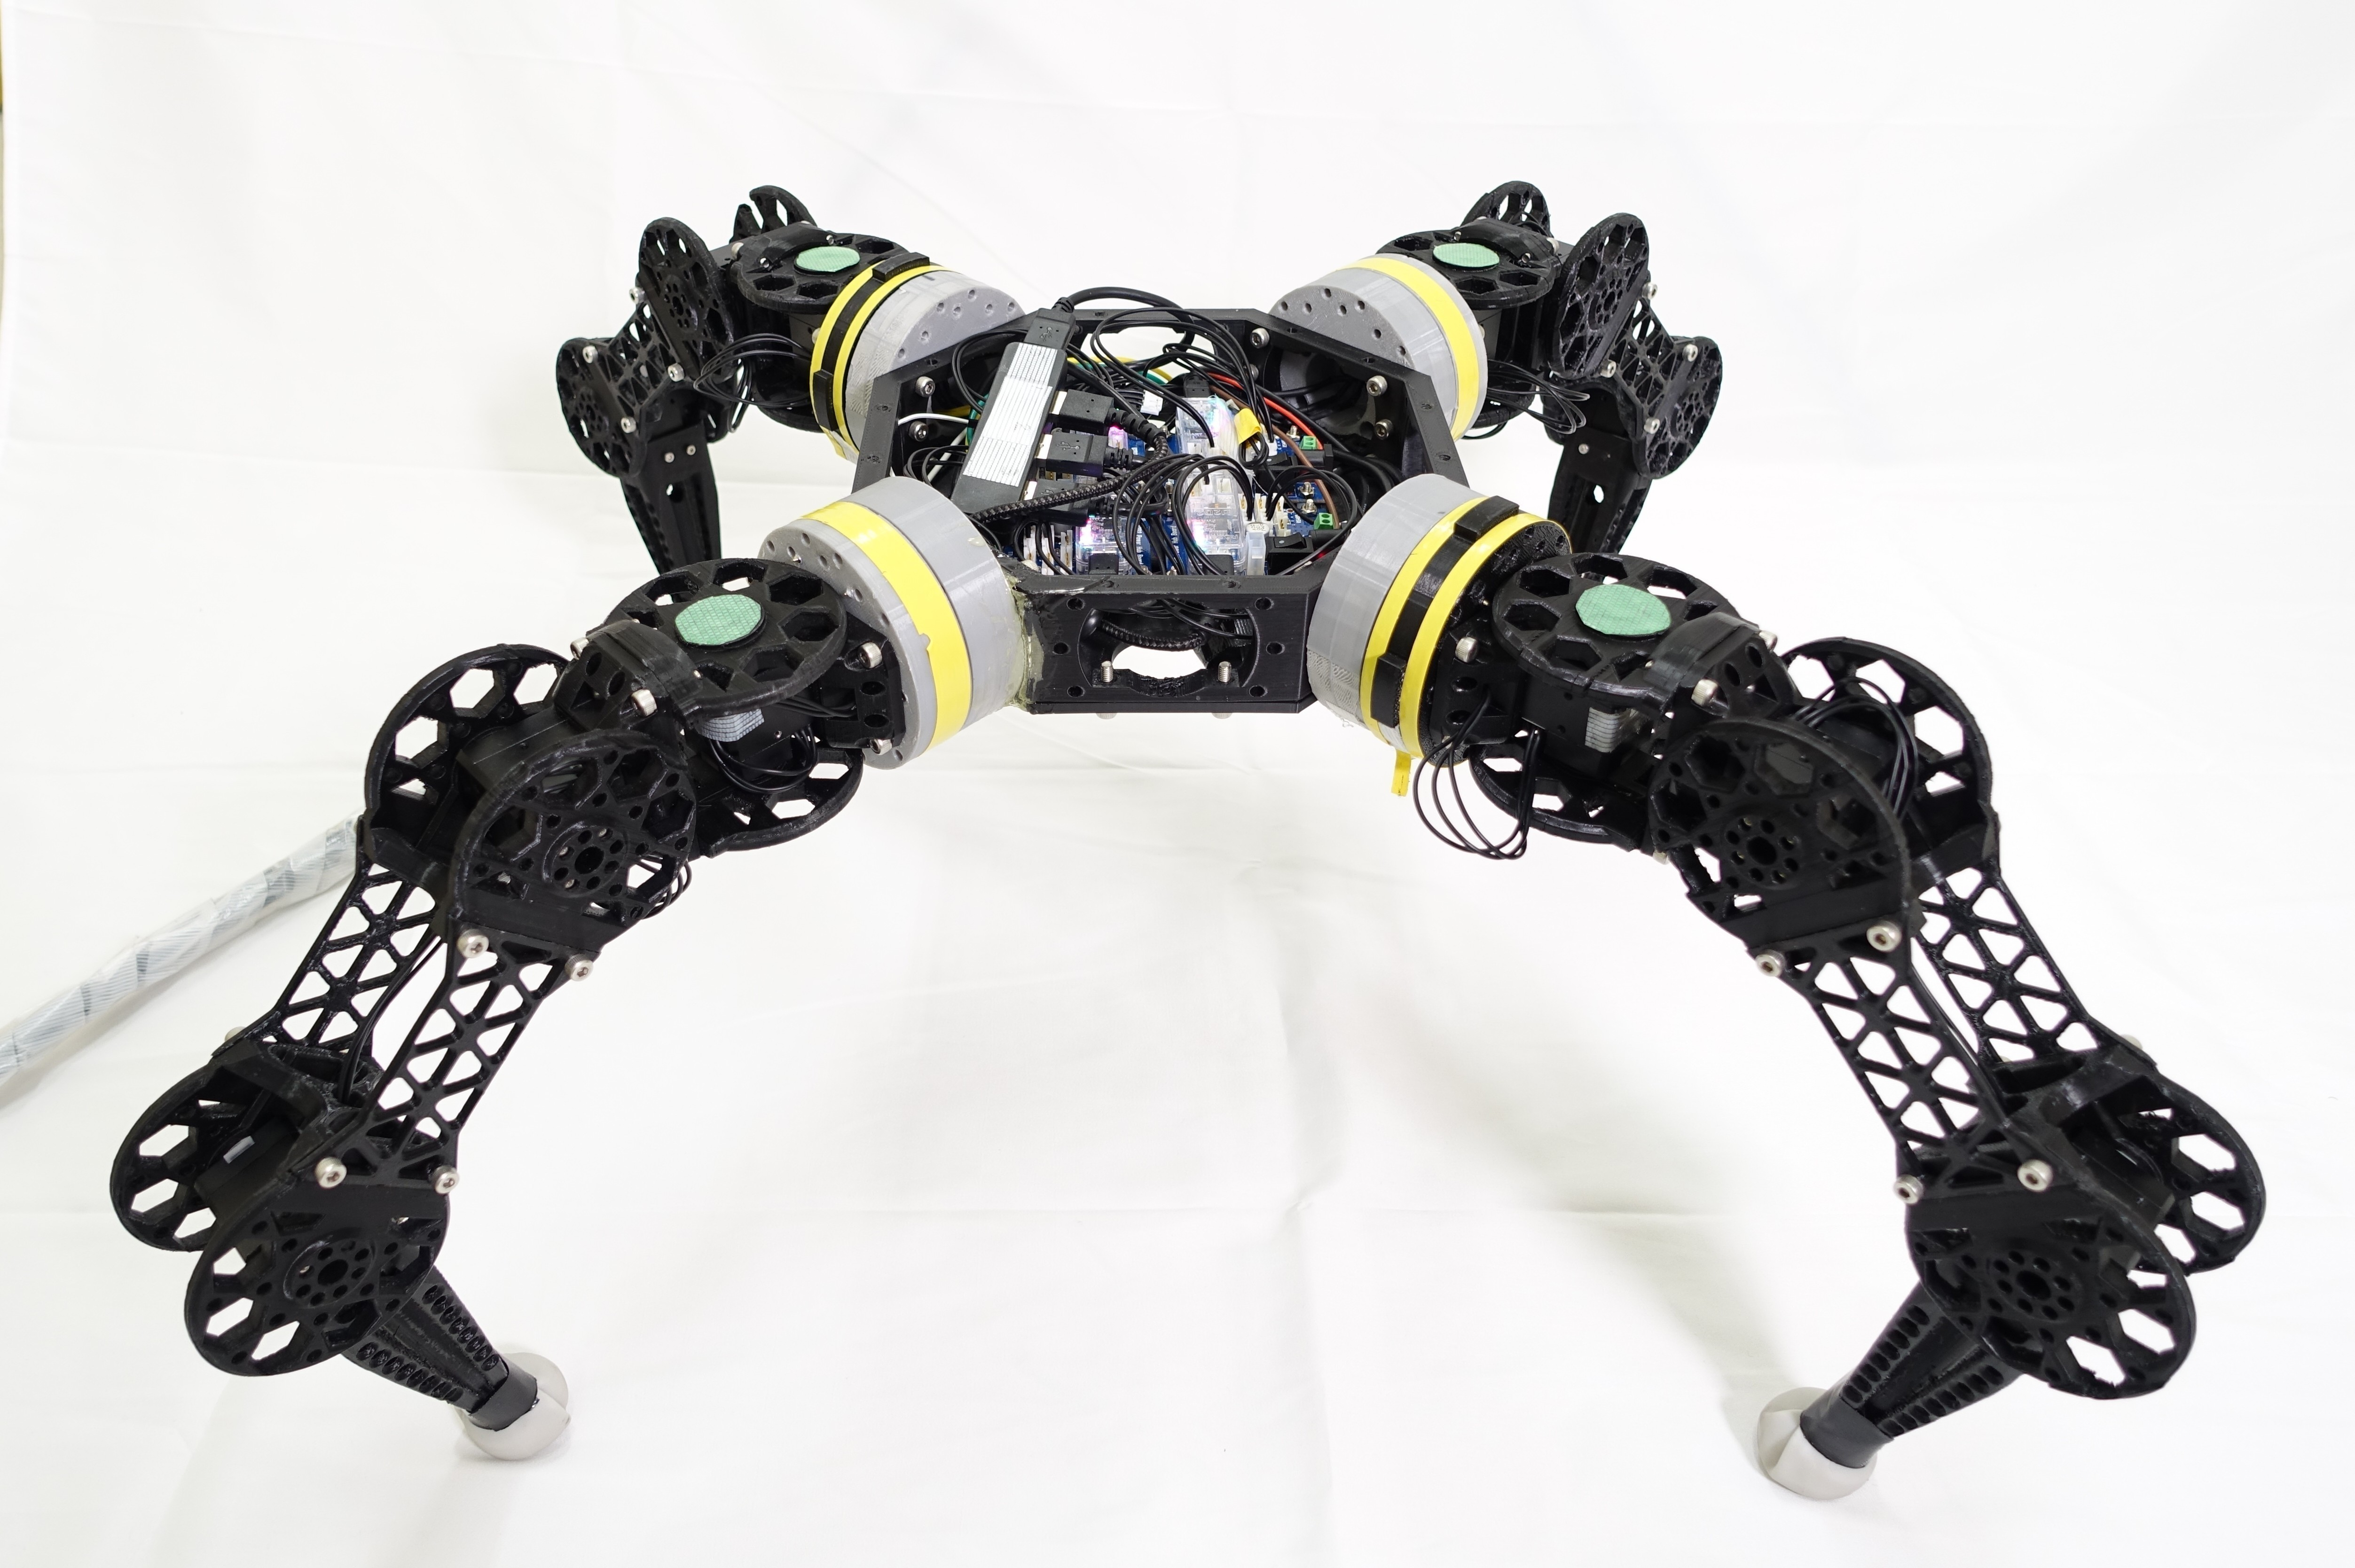
\includegraphics[width=40mm]{./fig/moonbot.jpg}
\caption{Moonbot assembly}\label{subfig1}
\end{center}
\end{subfigure}
 \begin{subfigure}{0.23\textwidth}
 \begin{center}
  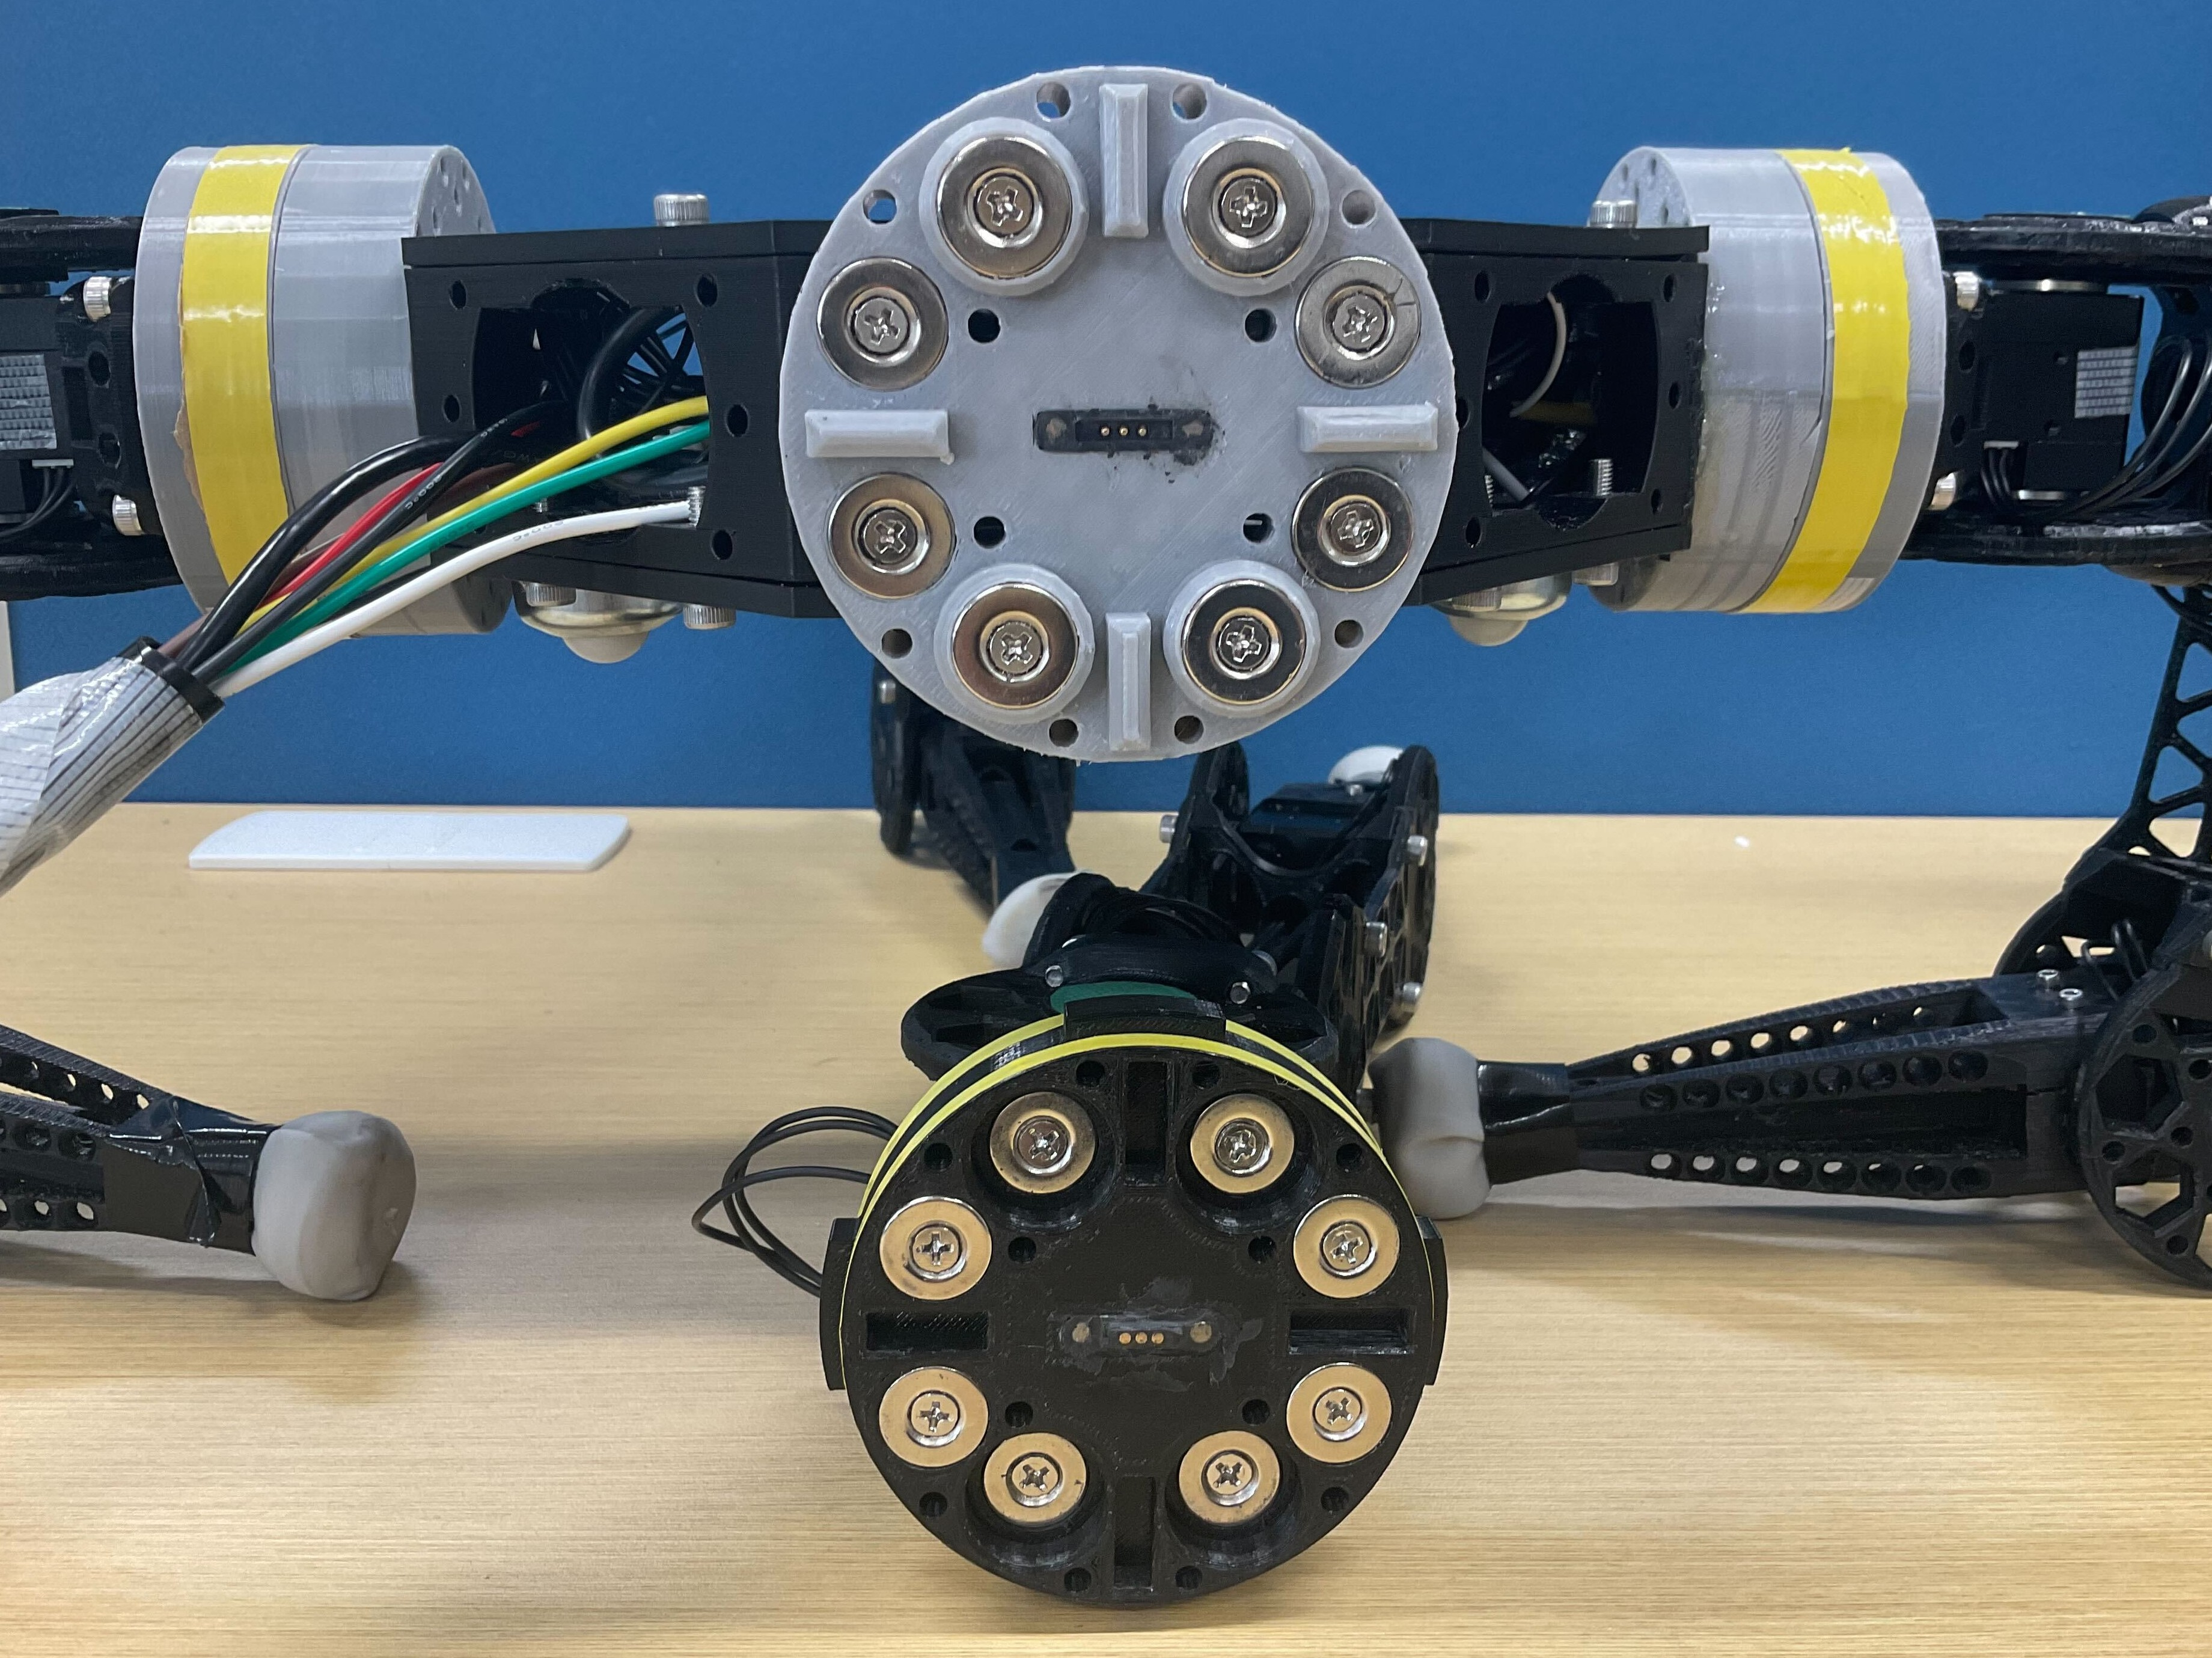
\includegraphics[width=35mm]{./fig/pogopin.jpg}
\caption{Pogo pin connection}
\label{subfig2}
 \end{center}
 \end{subfigure}
\vspace{-2mm}
\caption{Moonbot and magnetic connection with pogo pin}
\label{fig1}
\end{figure}
%%%

%%% Section 3 %%%
\section{Software Architecture and Control}
Moonbot, designed for lunar surface operation, relies on a robust software foundation to achieve seamless communication and precise control. This section provides insight into the software intricacies, emphasizing the use of ROS2 (Robot Operating System 2) \cite{ros2} as the primary tool for orchestrating communication among Moonbot's modular components.

Moonbot is controlled through the \texttt{ros2\_control} package \cite{ros2control}, offering a modular and extendable framework. Each leg operates as an independent entity, with its own controller. 

%%%
\subsection{Self-Recognition}
Moonbot's configuration can be changed by the attach and detach module via magnetic port. To select the strategy of control, the robot itself need to know the current configuration and also the type of connected module (e.g. yaw-pitch-pitch leg, gripper). Inspired from the design of Snapbot, the modular legged robot by Disney Inc. \cite{snapbot1} \cite{snapbot2}, connections of Moonbot are periodically checked by pinging the existing of specific ID of Dynamixel motors. \fig{fig2} shows the flowchart of modular connection algorithm. The controller of each leg connection is separately launched, after the connection is detected, the control package of the specific leg will be activated and status of the port is stated as ``connected". Finally, with the specific configuration, the robot selects the appropriate locomotion style. 
%%%
\begin{figure}[t]
  \centering
  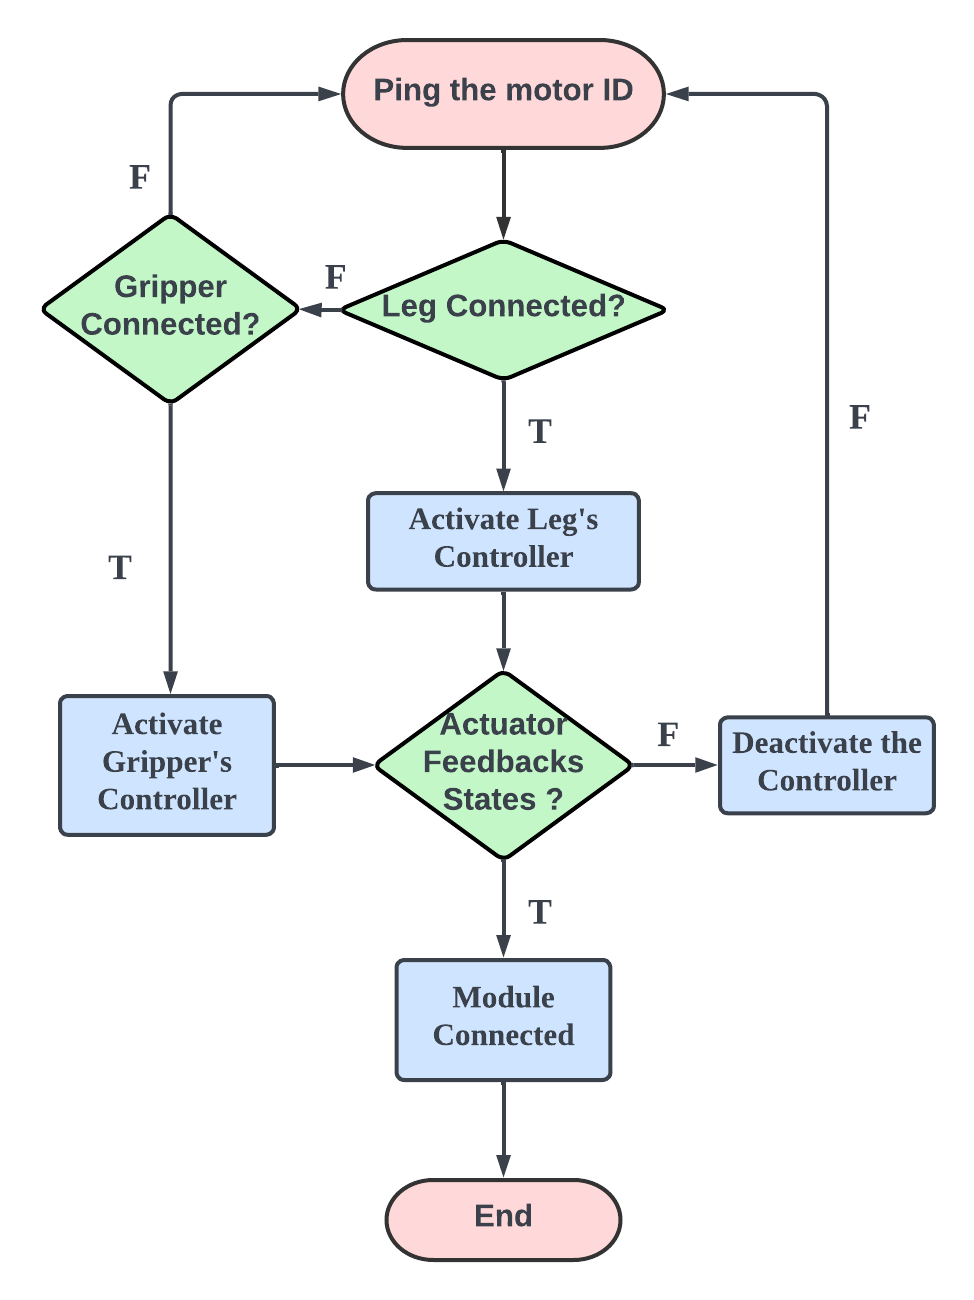
\includegraphics[width=65mm]{./fig/flowchart/flowchartcolor.png}
  \caption{Self-recognition algorithm for each connection.}\label{fig2}
\end{figure}
%%%
%%%
\subsection{Locomotion}
Moonbot's locomotion is mobilized through the integration of \texttt{ros2\_control} package. The joint trajectory controller is used to operate the multiple joints. The locomotion styles include crawling motion and walking motion.

\begin{figure}[ht]
  \centering
  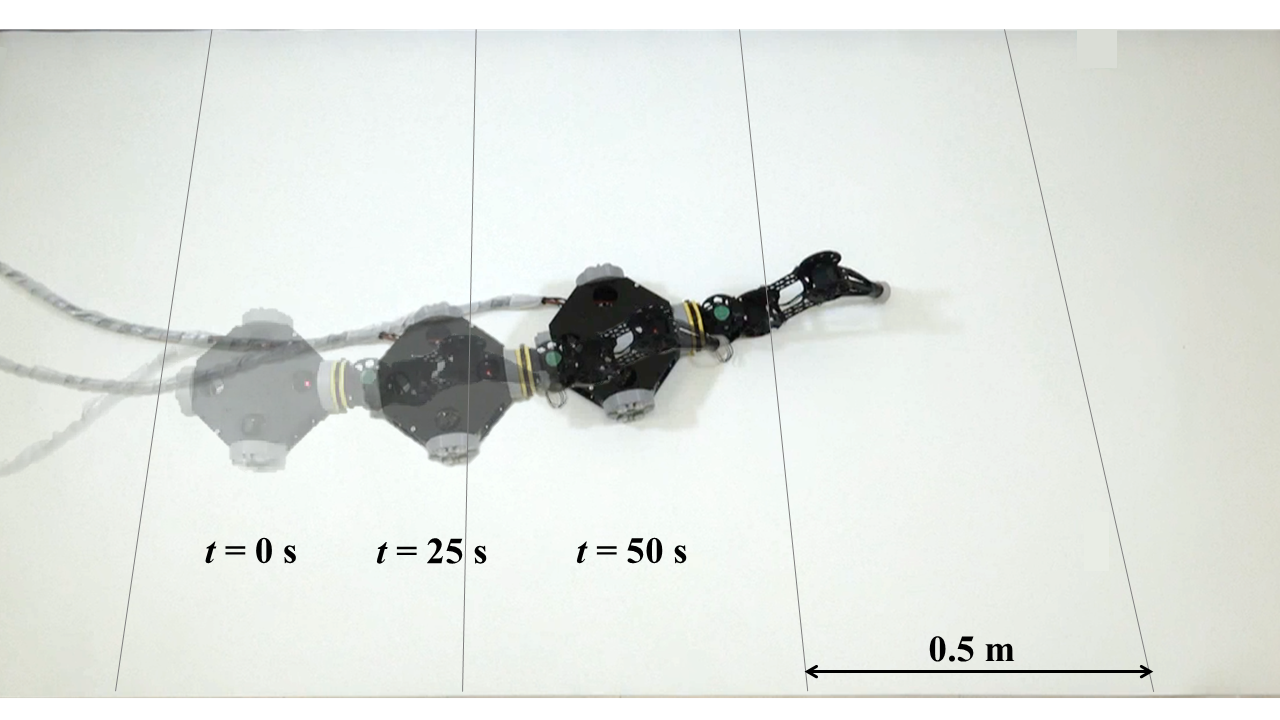
\includegraphics[width=60mm]{./fig/snapshot/single_snapshot_final.png}
  \caption{Snapshots of crawling motion for single-leg configuration.}\label{fig3singlesnap}
\end{figure}

\begin{figure}[ht]
  \centering
  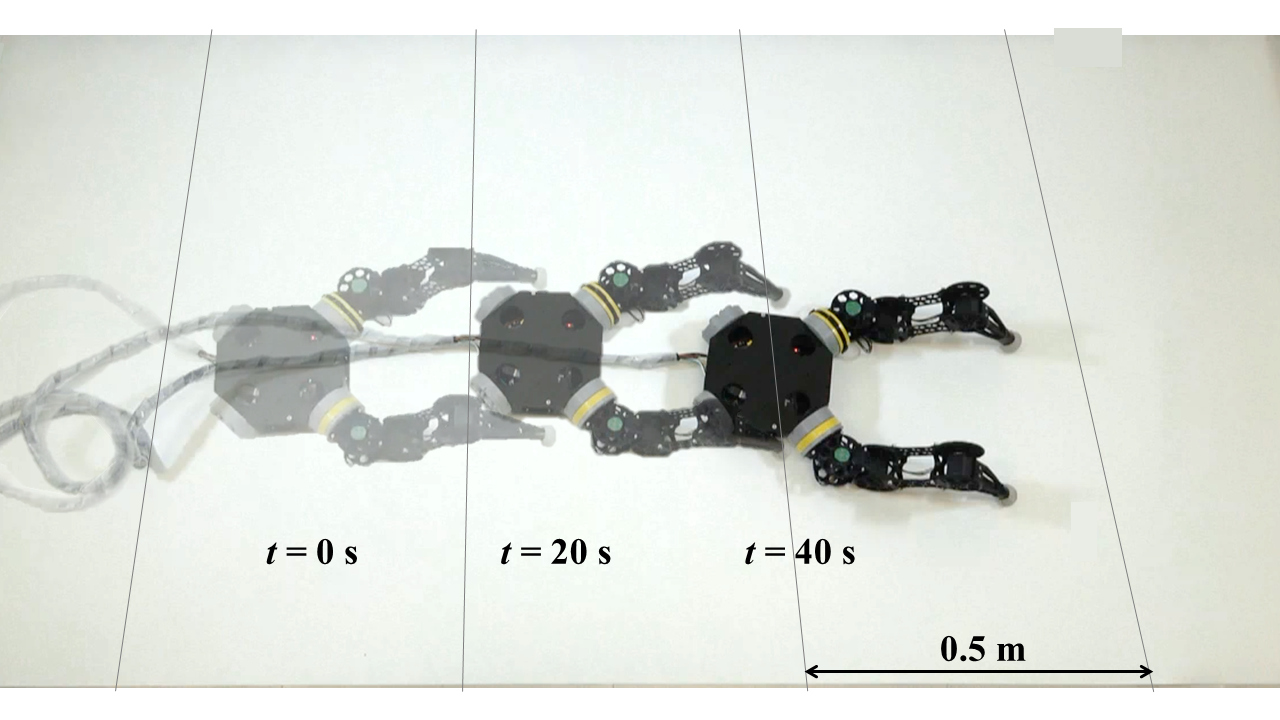
\includegraphics[width=60mm]{./fig/snapshot/double_snapshot_final.png}
  \caption{Snapshots of crawling motion for double-leg configuration.}\label{fig4doublesnap}
\end{figure}

% \begin{figure}[h]
%  \begin{subfigure}{0.15\textwidth}
%  \begin{center}
%   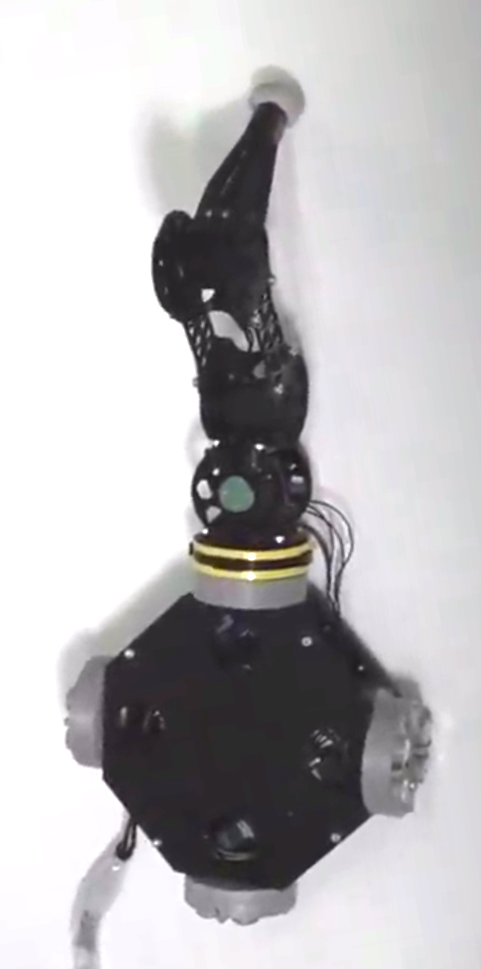
\includegraphics[width=14mm]{./fig/11.png}
% \caption{Neutral pose}\label{snapshot1.1}
%  \end{center}
%  \end{subfigure}
%  \begin{subfigure}{0.15\textwidth}
%  \begin{center}
%   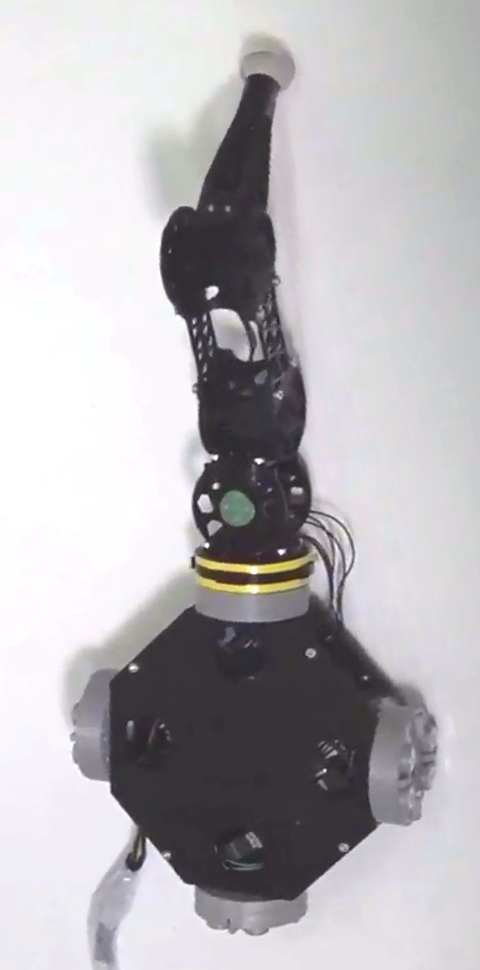
\includegraphics[width=14mm]{./fig/12.png}
% \caption{Stretch the leg}\label{snapshot1.2}
% \end{center}
% \end{subfigure}
%  \begin{subfigure}{0.15\textwidth}
%  \begin{center}
%   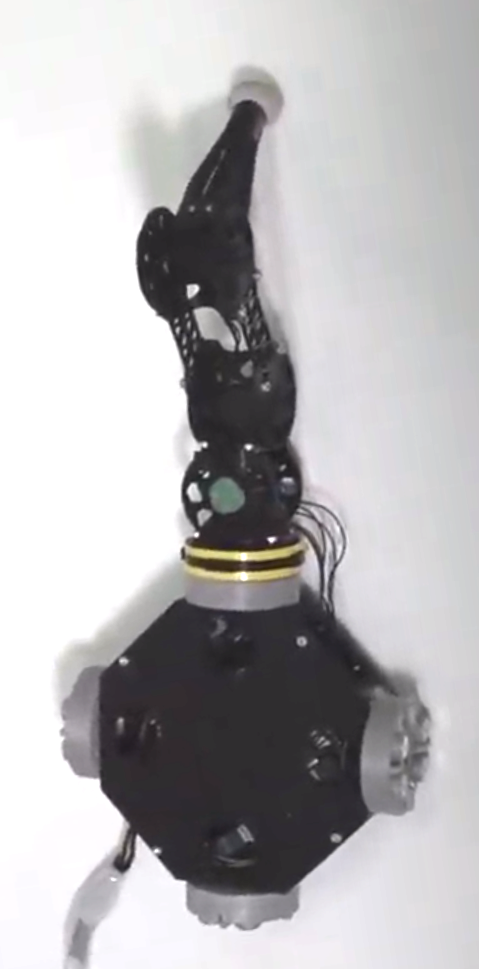
\includegraphics[width=14mm]{./fig/13.png}
% \caption{Pulling forward}\label{snapshot1.3}
%  \end{center}
%  \end{subfigure}
% \vspace{-1mm}
% \caption{Crawling motion for single-leg configuration}
% \label{snap1}
% \end{figure}

% \begin{figure}[h]
%  \begin{subfigure}{0.15\textwidth}
%  \begin{center}
%   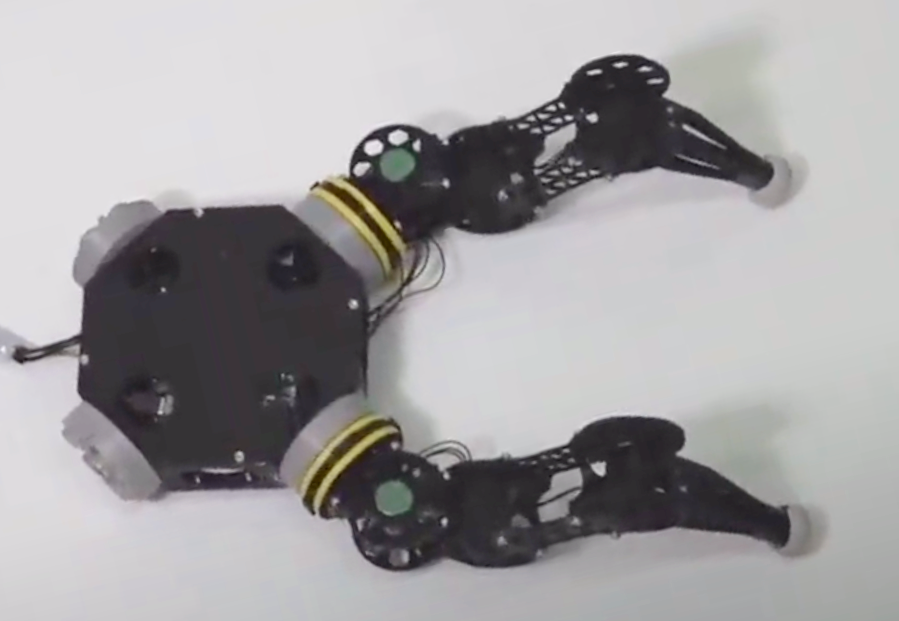
\includegraphics[width=23mm, angle=90]{./fig/21.png}
% \caption{Neutral pose}\label{snapshot2.1}
%  \end{center}
%  \end{subfigure}
%  \begin{subfigure}{0.15\textwidth}
%  \begin{center}
%   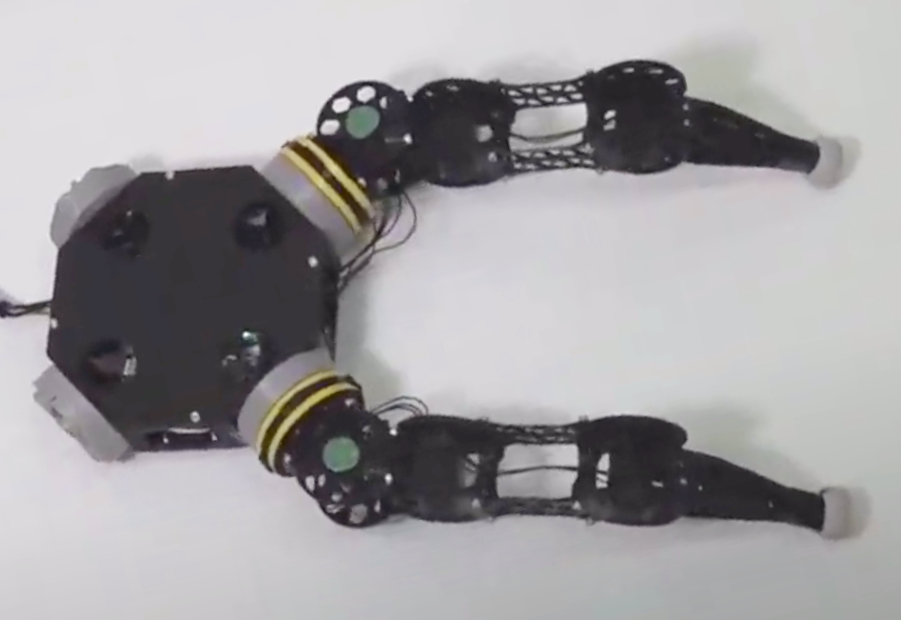
\includegraphics[width=23mm, angle=90]{./fig/22.png}
% \caption{Stretch the leg}\label{snapshot2.2}
% \end{center}
% \end{subfigure}
%  \begin{subfigure}{0.15\textwidth}
%  \begin{center}
%   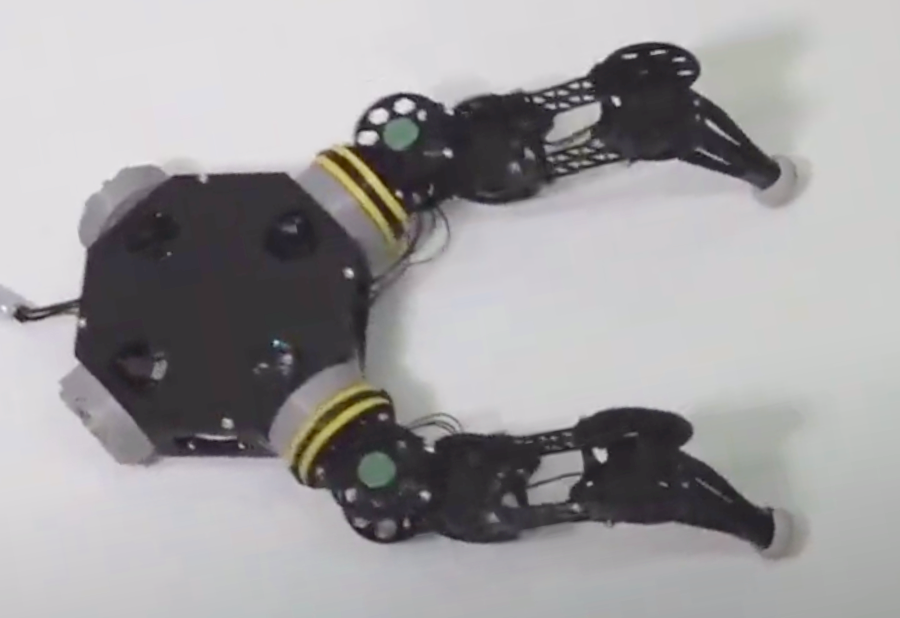
\includegraphics[width=23mm, angle=90]{./fig/23.png}
% \caption{Pulling forward}\label{snapshot2.3}
%  \end{center}
%  \end{subfigure}
% % \vspace{-1mm}
% \caption{Crawling motion for double-leg configuration}
% \label{snap2}
% \end{figure}

\label{enumerate}
\begin{enumerate}
\item \textit{Crawling Motion:}
Moonbot moves by crawling motion when operating with a single-leg configuration towards the direction of connected module. Extending its capabilities, two-legged and three-legged configuration, Moonbot move with the same style as single configuration, but higher power by more legs applied.\\

\item \textit {Walking motion:}
In full configuration, employing all four legs, is designed for versatile locomotion. Moonbot can perform both a crawl gait for static stability and a trot gait for a more dynamic walking motion as shown in \fig{fig5fullsnap}. 
\end{enumerate}
%%%

\begin{figure}[t]
  \centering
  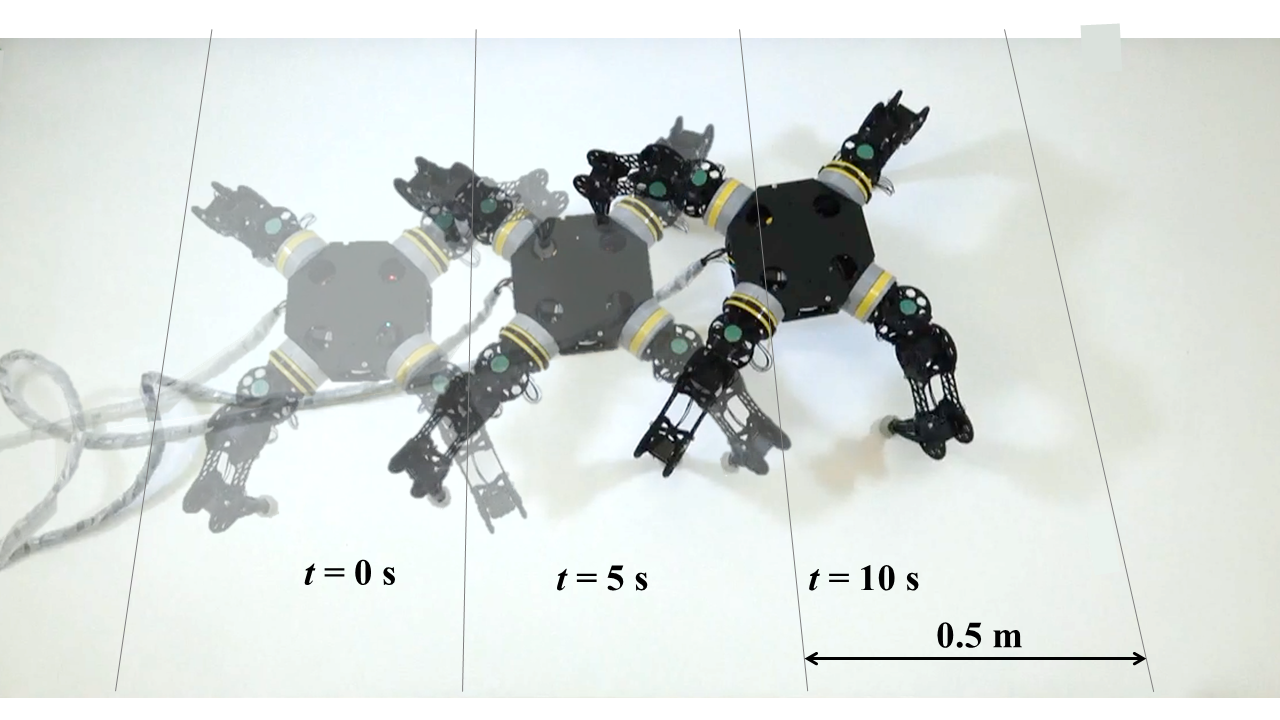
\includegraphics[width=70mm]{./fig/snapshot/full_snapshot_finaltrot.png}
  \caption{Snapshots of walking motion.}\label{fig5fullsnap}
\end{figure}

% \begin{figure}[t]
%   \centering
%   \begin{minipage}[ht]{0.14\textwidth}
%     \centering
%     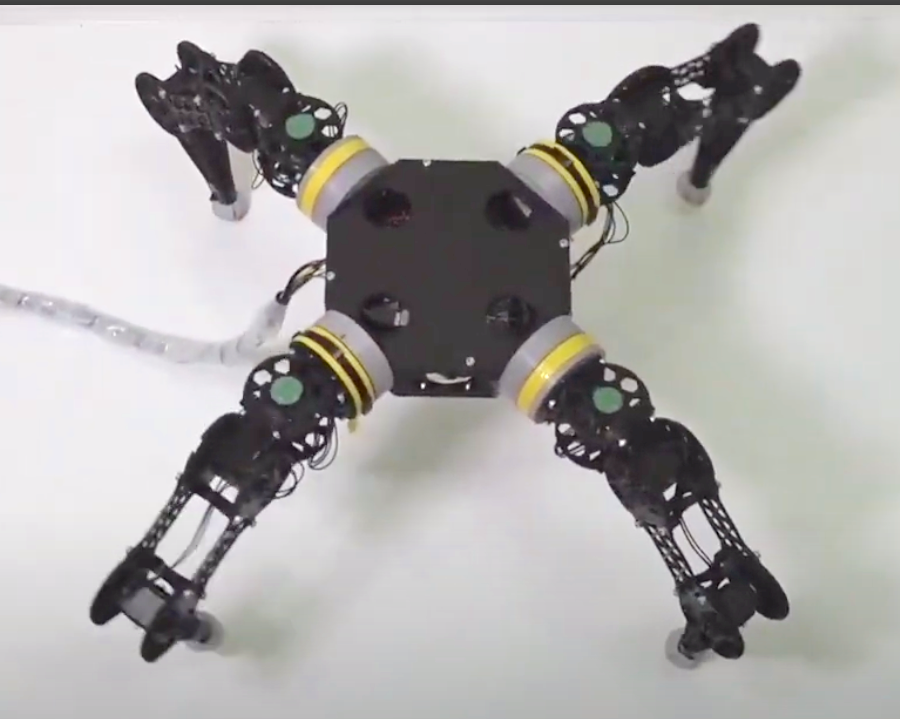
\includegraphics[clip, width=22mm]{./fig/40.png}
%   \end{minipage}
%   \begin{minipage}[ht]{0.14\textwidth}
%     \centering
%     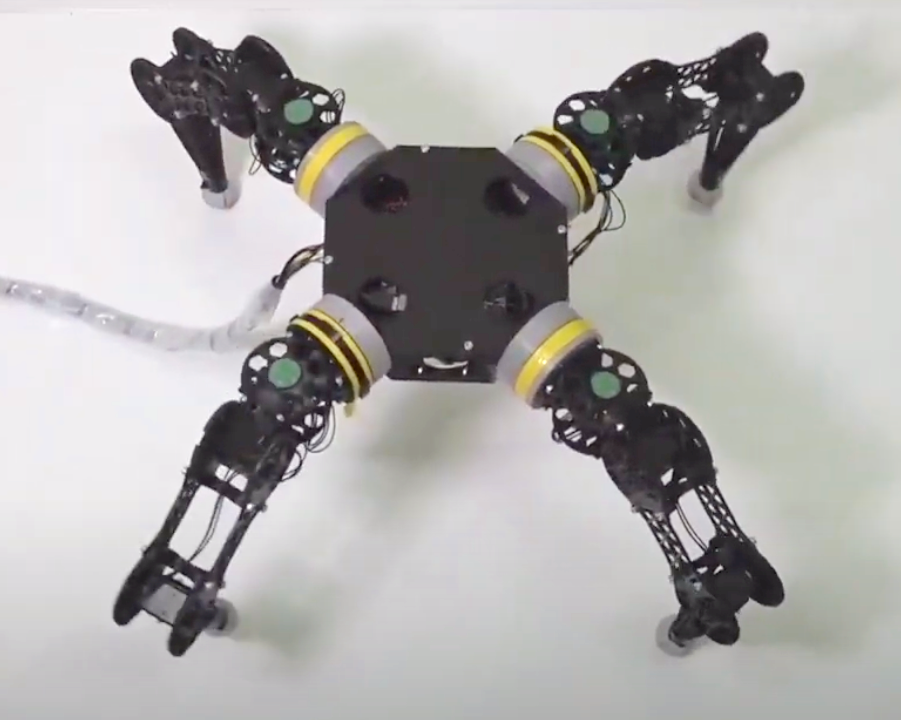
\includegraphics[clip, width=22mm]{./fig/41.png}
%   \end{minipage}
%   \begin{minipage}[ht]{0.14\textwidth}
%     \centering
%     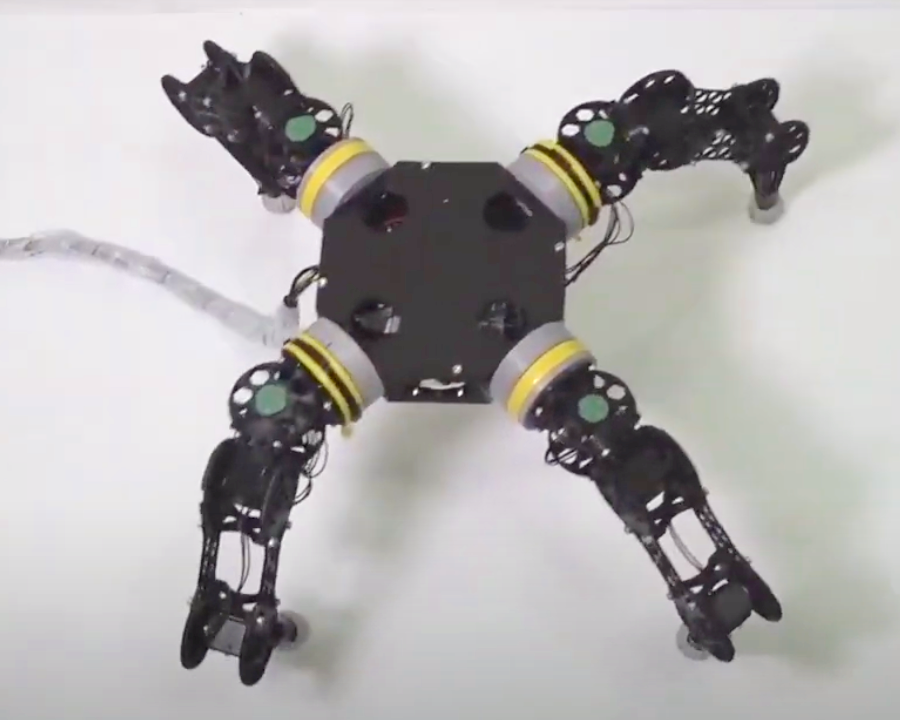
\includegraphics[clip, width=22mm]{./fig/42.png}
%   \end{minipage}\\
%   \begin{minipage}[ht]{0.14\textwidth}
%     \centering
%     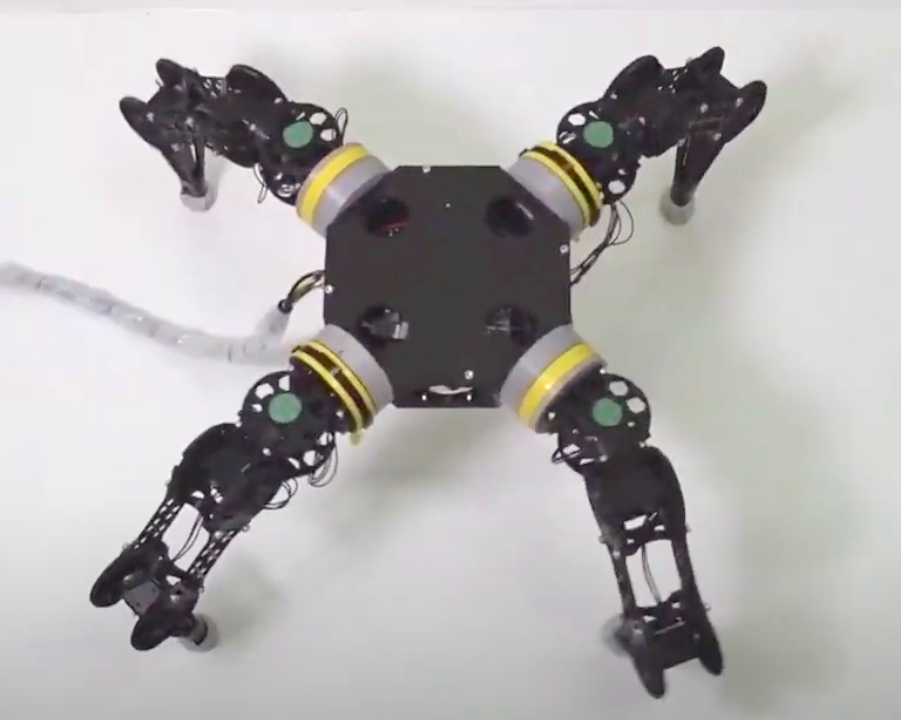
\includegraphics[clip, width=22mm]{./fig/43.png}
%   \end{minipage}
%   \begin{minipage}[ht]{0.14\textwidth}
%     \centering
%     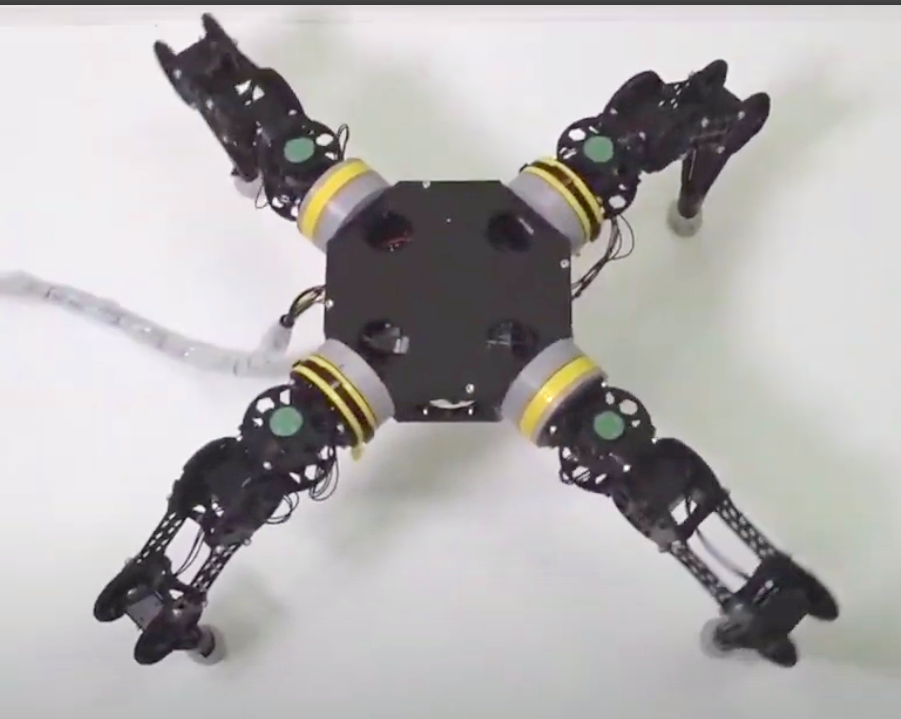
\includegraphics[clip, width=22mm]{./fig/44.png}
%   \end{minipage}
%   \begin{minipage}[ht]{0.14\textwidth}
%     \centering
%     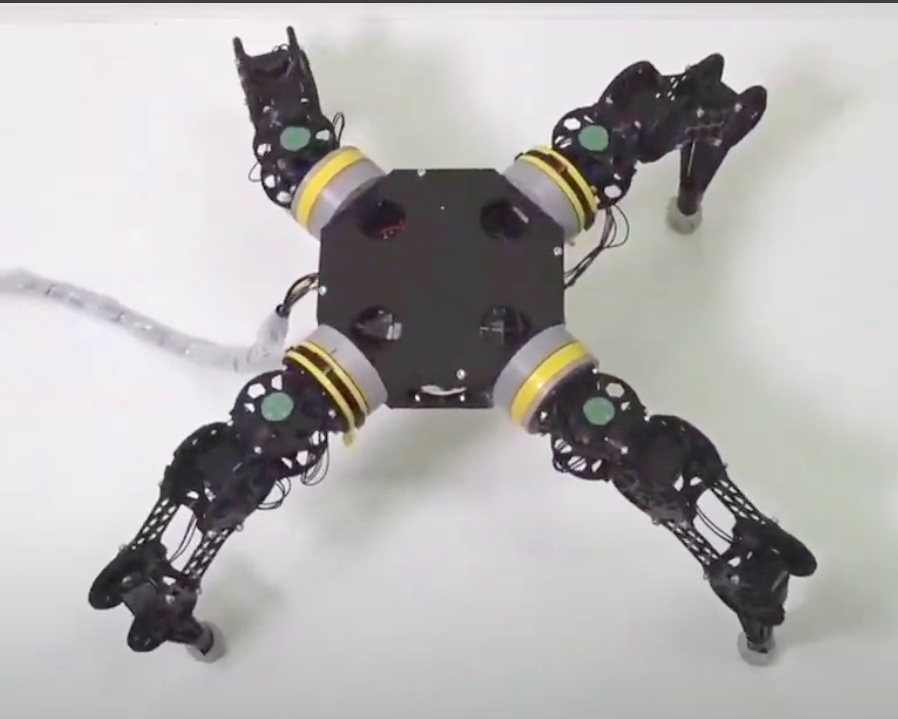
\includegraphics[clip, width=22mm]{./fig/45.png}
%   \end{minipage}\\
%   \begin{minipage}[ht]{0.14\textwidth}
%     \centering
%     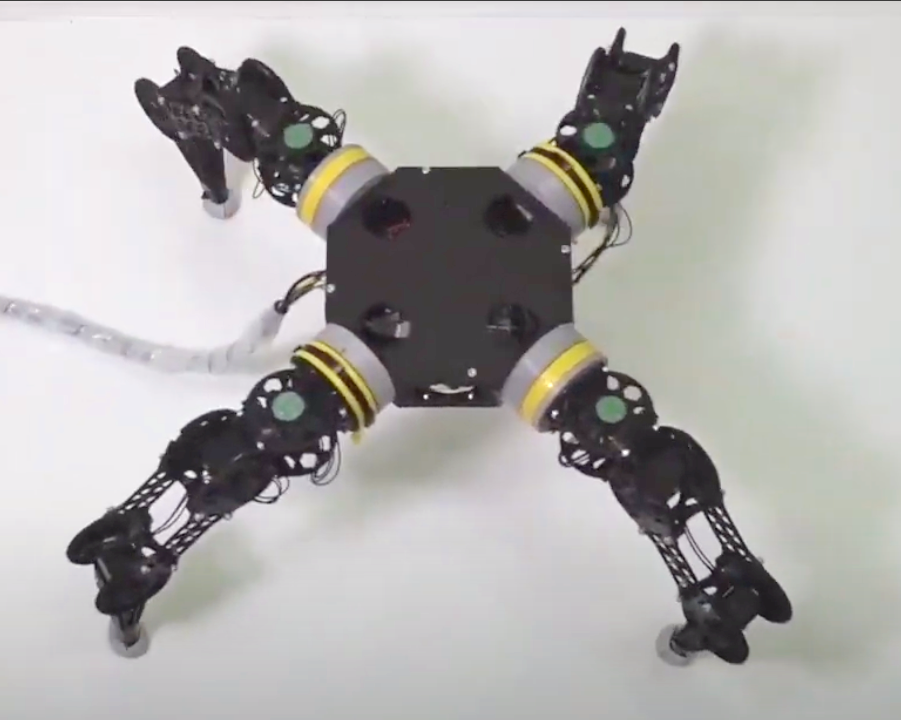
\includegraphics[clip, width=22mm]{./fig/46.png}
%   \end{minipage}
%   \begin{minipage}[ht]{0.14\textwidth}
%     \centering
%     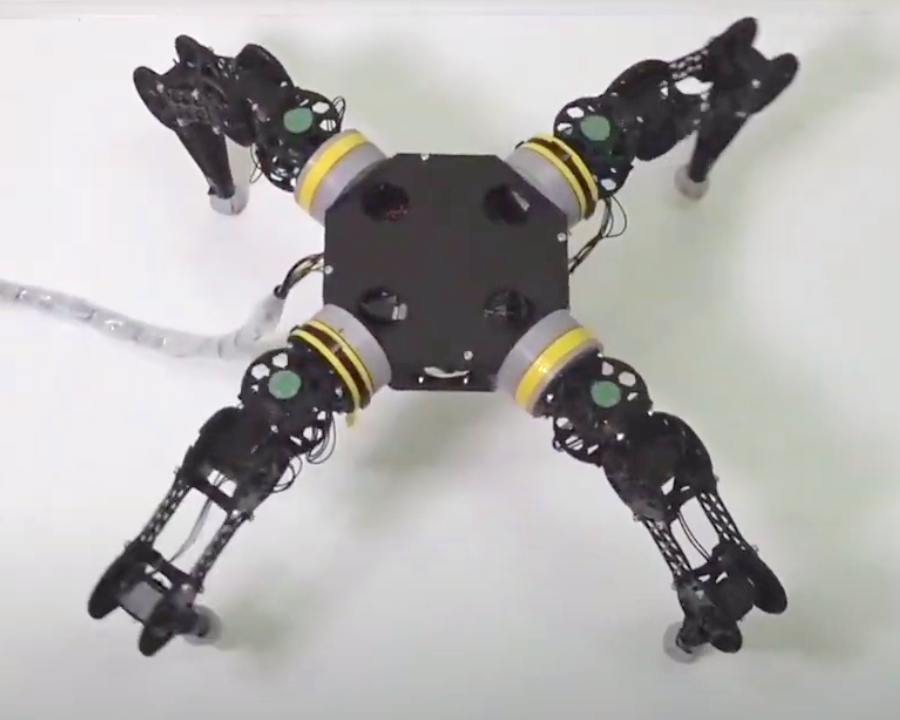
\includegraphics[clip, width=22mm]{./fig/47.png}
%   \end{minipage}
% \caption{Walking motion}
% \label{minipage}
% \end{figure}

%%% Section 6 %%%
\section{Conclusions}
\indent
Moonbot is a modular legged robot, embodying the self-recognition-based motion control. With modularity, Moonbot can adapt to various leg configurations.

The magnetic connections contribute to Moonbot's structural flexibility, while the integration of ROS2 in its software architecture ensures efficient self-recognition and versatile locomotion. 

Looking ahead, the goals of the Moonbot also include the implementation of Reinforcement Learning algorithms and proprioceptive sensing. This can advance the control strategies and enhance adaptability to diverse configurations and terrain. The target of the plan is to elevate the Moonbot's performance capabilities in the realm of modular legged robotics for space exploration.

%%%%%%%%%%%%%%%%%%%%%%%%%%%%%%%%%%%%%%%
%%%  2020.01.08 modified by Kentaro UNO
%%%  pBibtexを使ったものに書き換え
%%%%%%%%%%%%%%%%%%%%%%%%%%%%%%%%%%%%%%%

%\begin{thebibliography}{8}
%{\small
%\bibitem{No.1}
%\begin{spacing}{0.85}
%J. Walker, et al.,
%{\it``Qualification of Commercial Off-The-Shelf Components for a Lunar Rover Mission''},
% \textit{Proc. FSR2015}, \#41, 2015.
%%\end{spacing}
%\bibitem{No.2}
%%\begin{spacing}{0.85}
%S. Fuchs and G. Hirzinger,
%{\it``Extrinsic and Depth Calibration of ToF-cameras''}, \textit{Proc.CVPR 2008}, pp.1-6, 2008.
%\end{spacing}
%}
%\end{thebibliography}
\small
\section*{Acknowledgement}
\indent 
This work was supported by JST Moonshot R\&D Program, Grant Number JPMJMS223B.
\small 
%\begin{spacing}{0.85} %参考文献の行間を詰めたい場合はここをアンコメント.
%\bibliographystyle{./include/IEEEtranWithJP} %%% use customized Bibtex style file. 2020.01.08 modified by Kentaro UNO 
%%%%%%%%%%%%%%%%%%%%%%%%%%%%%%%%%%%%%%%%%%%%%%%%%%%
%%% for Japanese reference, use Bibtex style file downloaded from: https://github.com/YoshiRi/JPandENbst.git. 2020.03.22 modified by Kentaro UNO
%%%%%%%%%%%%%%%%%%%%%%%%%%%%%%%%%%%%%%%%%%%%%%%%%%%
\bibliographystyle{./include/IEEEtran}
% \bibliographystyle{plain}

\bibliography{./bibtex/reference}
%\end{spacing} %参考文献の行間を詰めたい場合はここをアンコメント.

\end{document}

